
\subsection{Waste Form Degradation Rate}
\label{sed:wfdeginv}


The sensitivity of peak dose rate to the waste form degradation rate was 
determined with respect to varying inventories of waste.

The sensitivity of repository performance to waste form degradation rate was
expected to vary according to the waste inventory. For cases in which the dominant dose contributing 
radionuclides have half-lives much shorter than the expected waste form lifetime, 
the waste form degradation rate is not expected to have an effect. So too, for 
cases in which the primary barrier to release, the slow diffusive pathway, 
dominates overall repository performance, the waste form engineered barrier was
expected to have a negligible effect on repository performance in comparison.

In the case of a clay repository, the effect of the long time scale of the 
diffusive release pathway was to dampen the potential effect of high waste form 
degradation rates. 

\subsubsection{Parametric Range}

These runs varied the waste form degradation rate and the waste inventory mass 
factor.  There were forty runs corresponding to eight values of the waste form degradation 
rate and five values of the mass factor.

The waste form degradation rate was varied over the eight magnitudes 
between $10^{-9}$ and $10^{-2} [1/yr]$. The inventory mass factor was varied 
over the five magnitudes between $0.001$ and $10.0 [-]$. 

\subsubsection{Safety Indicators}
Safety indicators for post closure repository performance have been developed by 
the \gls{UFD} campaign which utilize the inventory multiplier that was varied in 
this study \cite{nutt_generic_2009}. These indicators are normalized by a 
normalization factor (100 mrem/yr) recommended by the \gls{IAEA} as the limit to 
``relevant critical members of the public'' \cite{international_atomic_energy_agency_international_1996}. The functional form for 
this safety indicator for a single waste category, \gls{HLW}, is just 

\begin{align}
SI_{G} &= \left(\frac{\sum_{i=1}^{N}D_{G,i}(I_i, F_{d})}{100mrem/yr}\right)[GWe/yr].
\label{indicator}
\intertext{where}
SI_{G} &= \mbox{Safety indicator for disposal in media type G}[GWe/yr]\nonumber\\
N &= \mbox{Number of key radionuclides considered in this indicator}\nonumber\\
D_{G,i} &= \mbox{Peak dose rate from isotope i in media type G}[mrem/yr]\nonumber\\
F_{d} &= \mbox{Fractional waste form degradation rate}[1/yr].\nonumber
\end{align}

Tables \ref{tab:WFDegIndicatorsTcICsSeCl}, 
\ref{tab:WFDegIndicatorsPdSnZrNb}, and 
\ref{tab:WFDegIndicatorsActinides} report the safety indicators for 
various independent isotopes and, where applicable, their daughters. 

\begin{table}[h!]
\centering
\includegraphics[width=0.5\textwidth]{./chapters/nuclide_sensitivity/clay/WFDegAndInv/IndicatorsSolNonSorbing.eps}
\caption{Safety indicators for soluble, non-sorbing nuclides.} 
\label{tab:WFDegIndicatorsTcICsSeCl}
\end{table}

\begin{table}[h!]
\centering
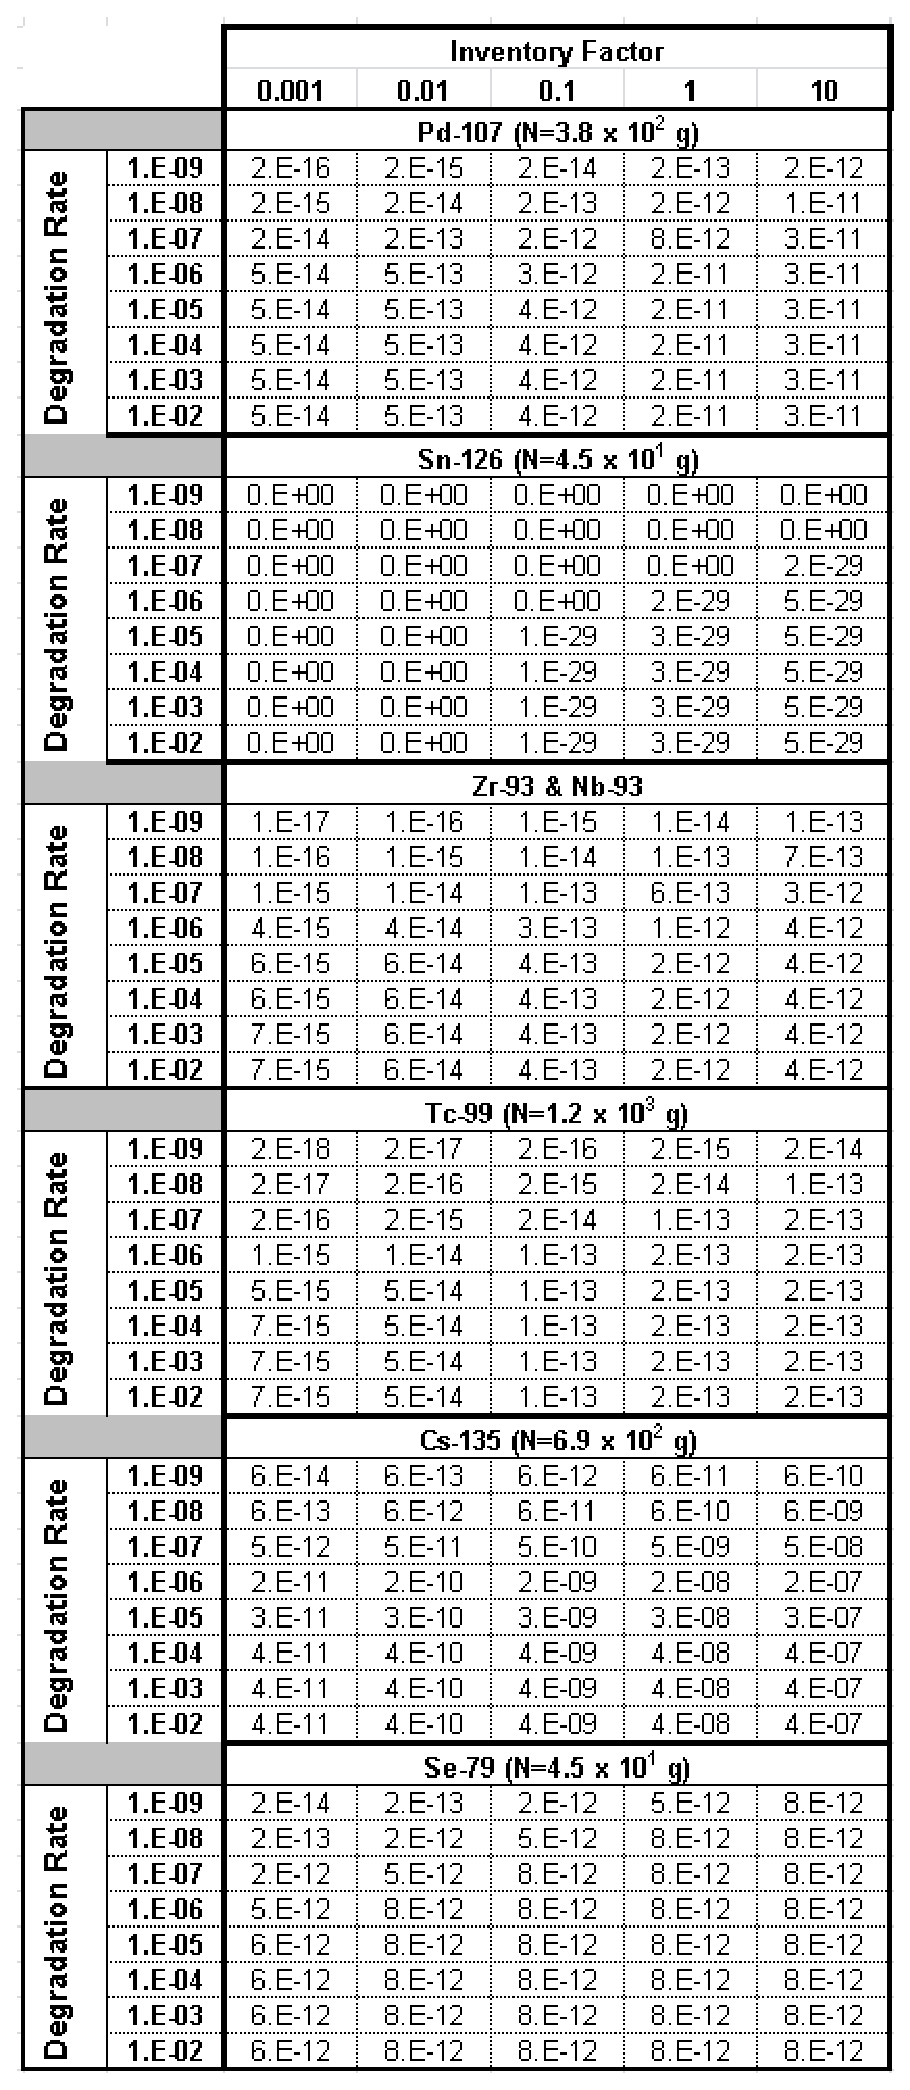
\includegraphics[width=0.5\textwidth]{./chapters/nuclide_sensitivity/clay/WFDegAndInv/IndicatorsSolLimSorbing.eps}
\caption{Safety indicators for solubility limited and sorbing nuclides.} 
\label{tab:WFDegIndicatorsPdSnZrNb}
\end{table}

\begin{table}[h!]
\centering
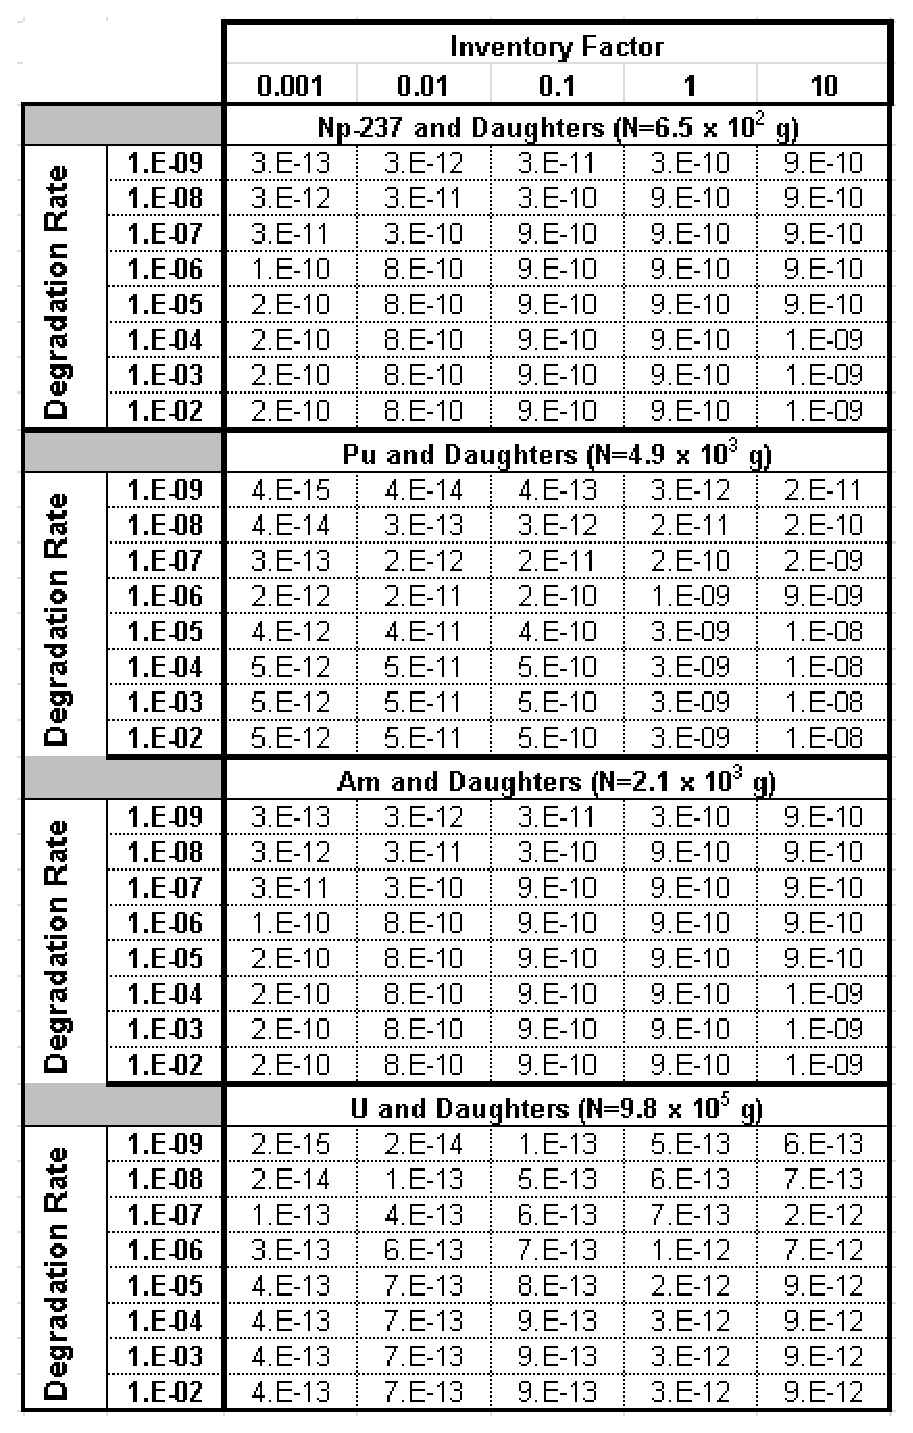
\includegraphics[width=0.5\textwidth]{./chapters/nuclide_sensitivity/clay/WFDegAndInv/IndicatorsActinides.eps}
\caption{Safety indicators for the actinides and their daughters.}
\label{tab:WFDegIndicatorsActinides}
\end{table}

\clearpage 
